\chapter{Conception et réalisation}
\begin{onehalfspace}

\newpage

\section{Conception}
\subsection{}
\subsection{Base de donnée}


\section{Réalisation à base d'un Cluster}


\section{Réalisation à base d'un mini PaaS}



\subsection{Supervision}

La Paas \emph{Deis} ne dispose pas d'un système de supervision intégré. Puisque les services déployés dans Deis fonctionnenet entièrement à l'intérieur des conteneurs Docker, cela signifie que les outils de supervision des conteneurs Docker devraient fonctionner avec Deis. L'on va utiliser les plus matures d'entre eux.


\subsubsection{Outils de supervision utilisés}


\subsubsubsection*{cAdvisor}



\begin{wrapfigure}{l}{3.5cm}
\centering

\includegraphics[scale=0.2]{chapitre4/assets/cadvisor}
\end{wrapfigure}
\noindent \emph{cAdvisor} (Container Advisor) fournit aux utilisateurs de conteneurs une vue de l'utilisation des ressources et des caractéristiques de performance de leurs conteneurs en cours d'exécution. C'est un démon, toujours en exécution, qui recueille, agrège, analyse, et exporte informations sur l'exécution des conteneurs. Plus précisément, pour chaque conteneur, il conserve l'historique de l'utilisation des ressources, les histogrammes des historiques complets d'utilisation des ressources et des statistiques du réseau. Ces données peuvent être exportées pour chaque conteneur ou pour toute la machine.

cAdvisor a un support natif pour les conteneurs Docker et devrait supporter à peu près tout autre solution de containérisation. Par ailleurs, cAdvisor fournit une interface utilisateur ainsi qu'une REST API.


\subsubsubsection*{Heapster}

Heapster est un projet open source de Google qui comble la limitation de cAdvisor qui supervise un seul serveur. Heapster receuille les données à travers les HTTP API fournit par les cAdvisor installés sur les serveurs, puis les stocker dans la base de donnée InfluxDB. Ainsi, Heapster est considéré comme un superviseur au niveau du cluster.

\subsubsubsection*{InfluxDB}

\begin{wrapfigure}{l}{3.5cm}
\centering

\includegraphics[scale=0.2]{chapitre4/assets/influxdb}
\end{wrapfigure}
\noindent Influxdb est une base de donnée distribuée destinée pour le stockage des métriques, des événements et des analyses de performances. Influxdb est simple à installer et à gerer, et rapide car il vise à répondre aux requête en temps-réel. En effet, chaque point de données est indéxé et diponible pour des requêtes qui retournent des réponses dans < 100 ms. Enfin, il dispose d'une HTTP API intégré qui va être sollicité par l'interface utilisateur Grafana.

\subsubsubsection*{Grafana}

\begin{wrapfigure}{l}{3.5cm}
\centering

\includegraphics[scale=0.3]{chapitre4/assets/grafana}
\end{wrapfigure}
\noindent Grafana est l'un des meilleurs projets open source pour la visualisation des données de mesure. Il fournit un moyen puissant et élégant pour créer, partager et explorer les données et les tableaux de bord à partir des bases de données de métriques. Grafana assure un support riche pour les bases de données Graphite, InfluxDB et OpenTSDB. Grafana sera utilisé pour visualiser les mesures stockées dans InfluxDB.


\subsubsection{Démarche d'installation}

Nous allons installer ce système de supervision dans un cluster Deis dont les serveurs fonctionne au-dessus de CoreOS. Comme c'est déjà mentionné, tous les services, sous CoreOS, sont installés en tant que conteneur. L'on trouvera les fichiers d'installations dans les annexes.  

\begin{itemize}
	\item cAdvisor doit être installé sur tous les serveurs du cluster; Heureusement, l'ordonnanceur Fleet effectue cette opération de façon automatique et scalable. En effet, il suffit de mentionner \emph{Global=true} dans le fichier d'installation;
	\item InfluxDB, Heapster et Grafana doivent être installé dans le même serveur. L'on exprime cette contrainte par \emph{X-ConditionMachineOf=influxdb.service}. Ainsi, Fleet va s'en sortir pour faire coexister les trois services.
\end{itemize}

\begin{figure}[H]
\centering
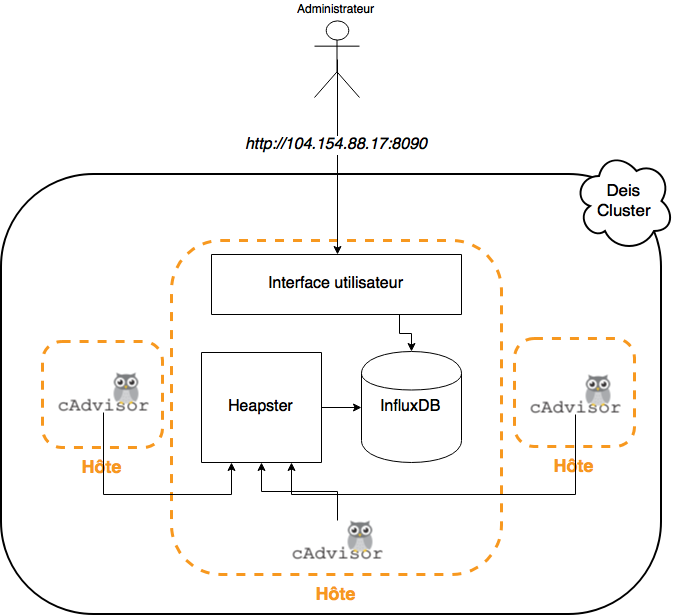
\includegraphics [scale=0.6]{chapitre4/assets/monitoring-cluster}
\caption{Architecture de la supervision}
\label{fig:}
\end{figure}


\subsubsection{Interfaces graphique}



\subsubsection{Supervision et scalabilité}

La scalabilité était toujours parmi nos aspirations tout au long de ce projet. Le système de supervision réalisé est conçu pour fonctionner de façon indépendante, complétement automatisée et hautement scalable. Nous allons prouver cela à travers ces deux scénarios:

\begin{itemize}
	\item Quand un nouveau service est lancé sur un des serveurs du cluster, cAdvisor se rendra compte de ce nouveau conteneur et va mettra à la disposition de Heapster les données qui va les stocker dans la base de données pour des consultations via l'interface graphique;
	\item Lors d'un pic de charge, on a intérêt à lancer les nouveaux conteneurs dans un nouveau serveur. On va tout d'abord lancer avec le fichier d'initialisation du cluster. Désormais, de façon automatique, le serveur appartient au cluster. Ainsi, les conteneurs lancés sur ce nouveau serveur sont supervisés automatiquement comme le décrit le scénario 1.
\end{itemize}

Grafana, l'interface utilisateur, sera disponible dans la machine dans laquelle \emph{Fleet} décide d'installer le trio Heapster, InfluxDB et Grafana. Cela signifie que Grafana peut changer de position dans le cluster à l'improviste et n'aura donc pas une adresse IP pour y accéder. Comme perspective, il serait préférable de mettre en place une sorte de proxy par lequel on accéde à Grafana partout où il soit.

\subsection{Sécurité avec le protocole \acrshort{ssl}/\acrshort{tls}}

C'est un système qui permet d'échanger des informations entre 2 ordinateurs de façon sûre. SSL assure 3 choses:

Confidentialité: Il est impossible d'espionner les informations échangées.
Intégrité: Il est impossible de truquer les informations échangées.
Authentification: Il permet de s'assurer de l'identité du programme, de la personne ou de l'entreprise avec lequelle on communique.
SSL est un complément à TCP/IP et permet (potentiellement) de sécuriser n'importe quel protocole ou programme utilisant TCP/IP.

\subsection{Messages logs}




\end{onehalfspace}
